% 
%jff-notes
%
\documentclass[11pt]{article}
\usepackage[pdftex]{graphicx}
\usepackage{amssymb}
\usepackage{latexsym}
%\usepackage{relsize}
\usepackage{textcomp}
%processed for 10 pt 
%\documentstyle[epsf,psfig]{article}
%\documentstyle[epsf]{article}
\oddsidemargin 0pt
\topmargin -0.0cm
\textwidth 6.2in
\textheight 8.5in
\baselineskip 18pt
%\renewcommand{\baselinestretch} {1.5}
\newenvironment{nitemize}
   {\begin{list}{\begin{math}\bullet\end{math}}%
      {\setlength{\leftmargin}{5mm}
       \setlength{\topsep}{1mm}
       \setlength{\parsep}{0in}
       \setlength{\itemsep}{.7mm}}}%
   {\end{list}}

\newcommand{\fract}[2]{\frac{\textstyle #1}{\textstyle #2}}
\newcommand{\trans}[3]{#1 \stackrel{#2}{\longrightarrow} #3}
\newcommand{\notrans}[3]{#1 \stackrel{#2}{\not\! \longrightarrow} #3}
\bibliographystyle{plain}
\begin{document}
\title{A simple PSK plugin for SDRuno}
\author{
Jan van Katwijk\\
Lazy Chair Computing \\
The Netherlands\\
{\em J.vanKatwijk@gmail.com}}
%\date{}
\maketitle
%\baselineskip 22pt
\ \\
\ \\
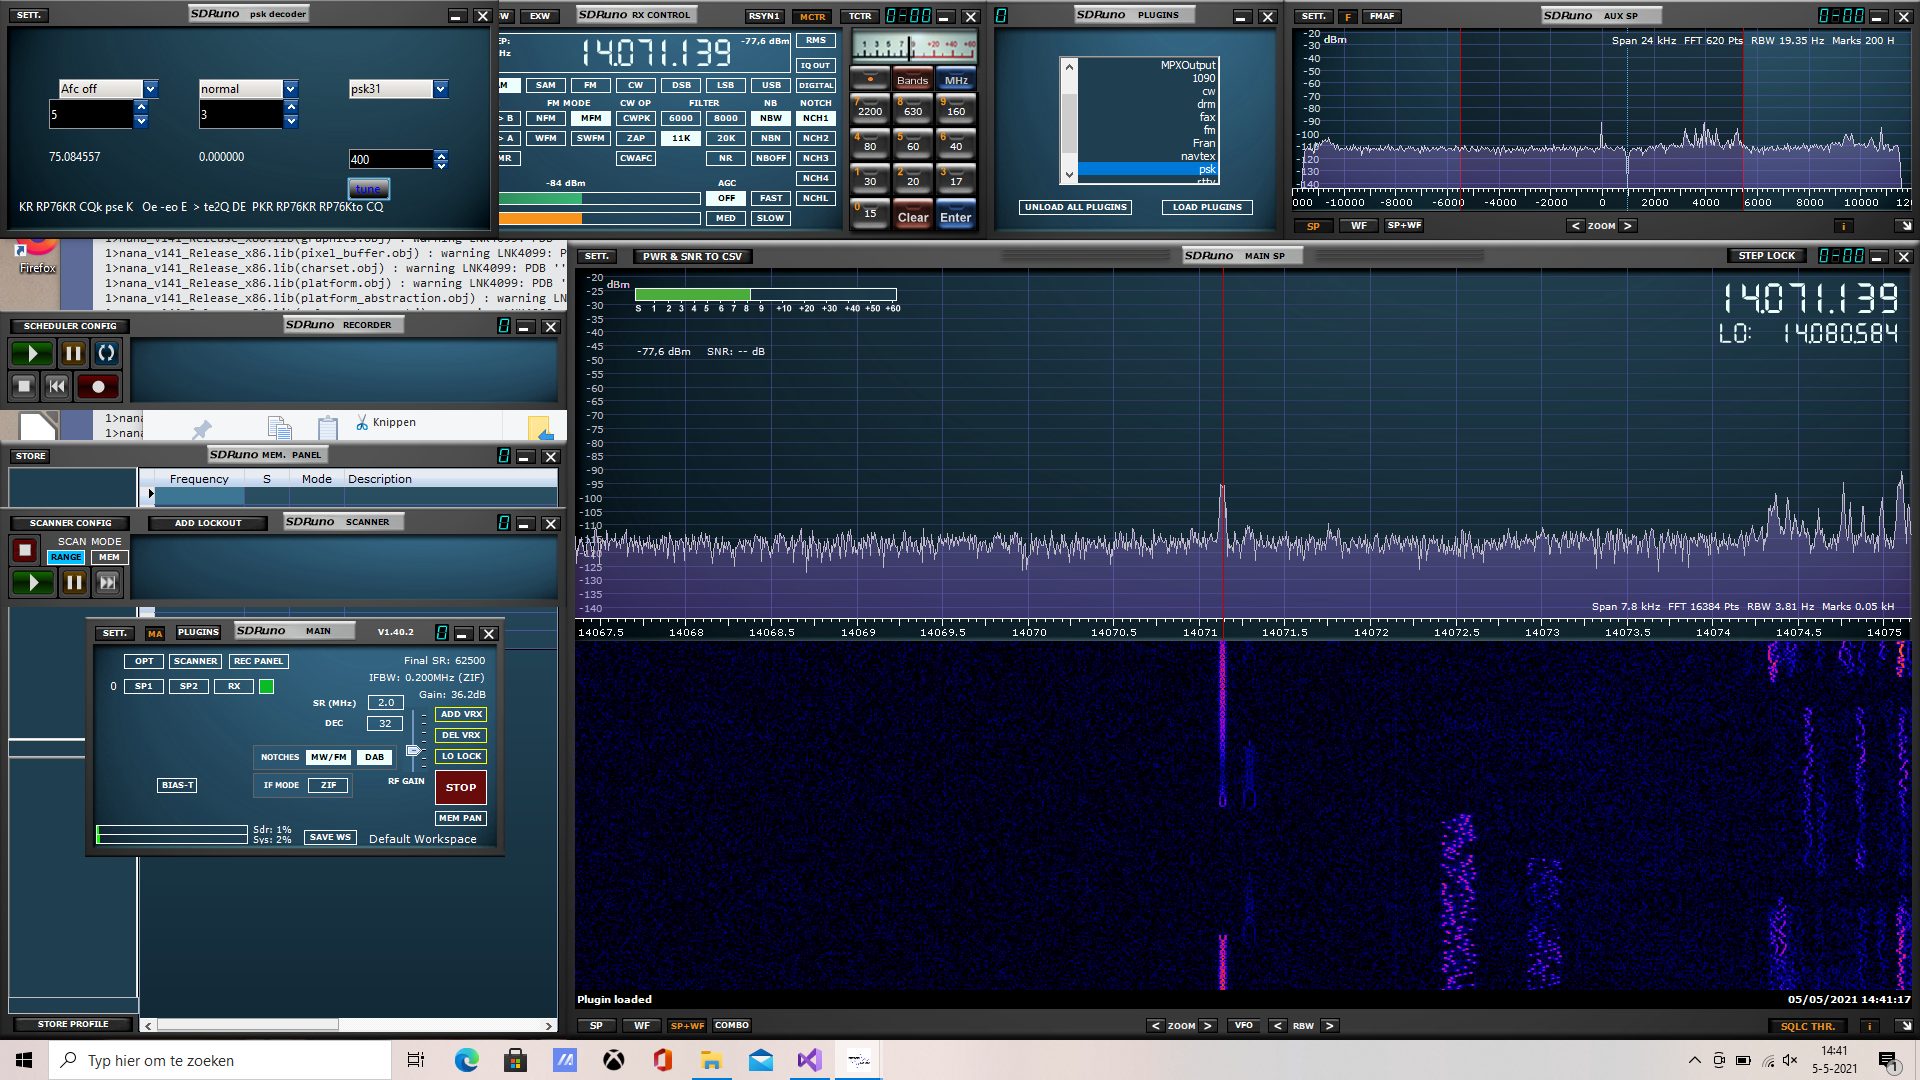
\includegraphics[width=140mm]{psk-example.png}
\ \\
\section{Introduction}
The SDRuno psk plugin is a simple plugin to decode a psk signal that
is tuned to. The current version supports BPSK31, BPSK63, and BPSK125.

PSK is less popular than about 5 to 10 years ago, nevertheless, the region
just above 14070 KHz usually contains quite some amateur calls using the
mode.

\section{Settings}
psk is a signal with a small footprint, the width used on  the band is
less than 50 Hz. The decoder therefore works with an intermediate
samplerate of 2000 samples/second. Since the minimal samplerate for the
SDRplay family is 2000000, a lot of decimation has to be done.
\par
This implementation requires an input sample rate of 62500 samples/second,
this requires the setting of the mainwidget to a samplerate of 2000000,
and a decimation of 32, as shown in the picture
One should realize that the SDRuno spectrum display shows a band of 62.5
KHz, the advantage is that one sees a lot of signals, the disadvantage
is that precise tuning, based on the view on the spectrum is not easy.

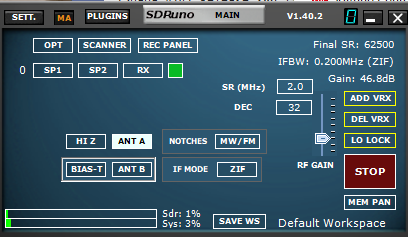
\includegraphics[width=100mm]{main-widget.png}

The plugin generates an audiotone of 800 Hz + the tuning offset,
the sound is output with a rate of 48000, setting "AM" in the RX control window
will set this rate.

\section{Tuning}
As said, psk is a signal with a small footprint, and since many of
the amateur transmissions are brief messages (such as CQ CQ ...), tuning
requires some training.
\par
What is really helpful here is the auxiliary spectrum display, the widget
can be enlarged, and one may zoom in such that one may view a spectrum
with a width of app 1 KHz.

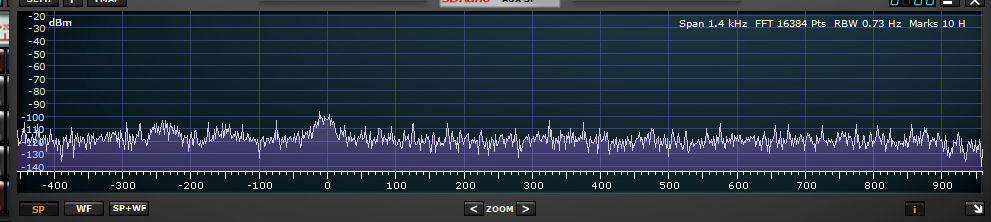
\includegraphics[width=100mm]{auxiliary-spectrum-display.png}

The way to tune is in two steps
\begin{itemize}
\item coarse tuning with the mouse on the main spectrum display;
\item fine tuning with the mouse controlled numerical display until the
psk signal is aboce the '0' in the auxiliary spectrum display.
\end{itemize}

\section{The plugin}
The plugin widget  is shown in the picture

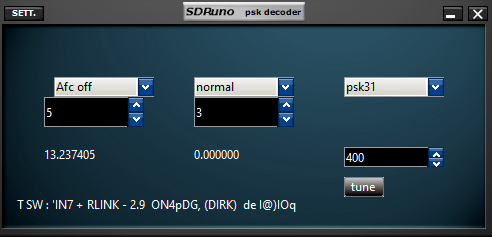
\includegraphics[width=100mm]{psk-plugin-widget.png}

The widget has three control comboboxes, and two spinboxes.

\begin{itemize}
\item the combobox, with {\em Afc on} on the picture, controls the afc. 
It just has two options {\em Afc on}, or {\em Afc off}. If "on", the
frequency offset used for correcting the measured frequency offset is
in the right label, here -4.7... Hz;
\item the combobox, with {\em normal} on the picture, let chose between
normal and inverse decoding;
\item the combobox, with {\em psk31} on the picture, controls the decoding mode.
As said, current modes are restricted to bpsk modes, in a later stage
the qpsk modes might be added.
\item the spinbox to the left tells the filter depth used for eliminating
the noise in the signal\footnote{the filter is a low pass FIR filter with
a degree that is twice the indicated number + 1. Of course a lot of filtering
was already done to get a reasonable clean signal};
\item the spinbox to the right sets a squelch level, below which there
is no decoding.
\end{itemize}

The number label to the left, below the filter depth indicator,
here with a value of 55...,
shows the "quality" of the decoding of the signal. As usual
with this kind of indicators, 100 is best.

The bottom line of the widget is reserved for the decoded signal. Note that
bpsk does not provide an error correction mechanism, and garbage may be shown.
\end{document}


